\subsubsection{Pulsoximeter} \label{pulsoximeter-1}

Als Pulsoximeter kam bei dem Projekt durchgehend der MAX30102 von der Firma Maxim Integrated zum Einsatz. Bei diesem Bauteil handelt es sich um ein schon mit dem MAX30100, sowie der dazugehörigen Peripherie, bestücktem Board(siehe Abbildung 3.2.2.1). Der MAX30102 wird wie auch der Temperatursensor über den I2C-Bus mit unserem Messboard verbunden.

\begin{figure}[H] \centering
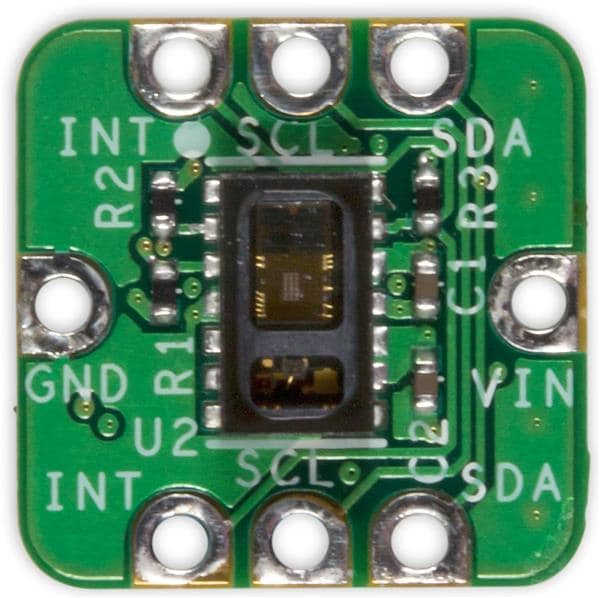
\includegraphics[width=\textwidth]{Images/MAX30102.png} 
\vspace{-0.3cm} 
\caption{Abb. MAX30102-Sensorboard. Vollständig vom Hersteller bestückt und bereit zur Verwendung}
\label{fig-elise} 
\end{figure}

Die Datenübertragung erfolgt wie auch beim MLX90614 mit einer Rate von  100.000 kbit/s. Der Sensor selbst verfügt über einen 16-Ebenen tiefen FIFO, in dem die Werte gespeichert und über den I2C-Bus auch ausgelesen werden können. Der Sensor selbst verfügt über LEDs (rot und infrarot), für die sowohl der Betriebsstrom, zwischen 0 und 50 mA,, als auch die Pulsbreite zwischen 200mirkos und 1,6mikros über den I2C-bus programmiert werden können. Abbildung Y zeigt das Systemdiagramm des MAX30102 auf dem die Funktion des Sensor aufgeführt ist. So wird die Messstelle von den auf dem Messboard befindlichen LEDs angeleuchtet, und dann wird mittels einer Photodiode der Reflektierte Anteil des Lichtimpulses gemessen.

\begin{figure}[H] \centering
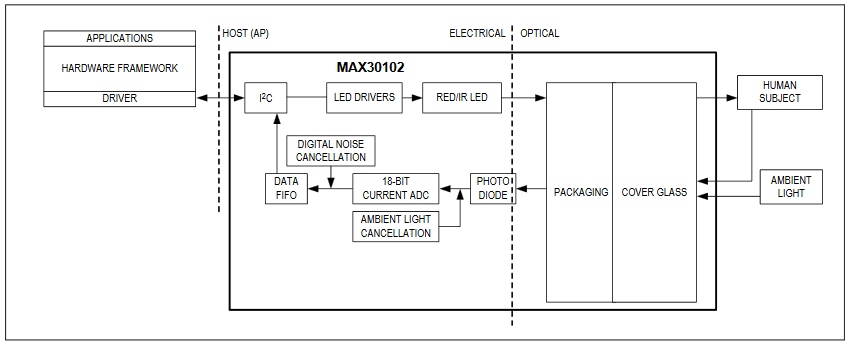
\includegraphics[width=\textwidth]{Images/Systemdiagramm.png} 
\vspace{-0.3cm} 
\caption{Abb.  Systemdiagramm des MAX30102.}
\label{fig-elise} 
\end{figure}

Dabei sind selbst Funktionen zur Unterdrücken von Umgebungsbeleuchtung und Rauschen schon auf dem Messboard enthalten.

Das Board kam in der gegebenen Fassung in allen Prototypen und Messungen zum Einsatz. Die einzige Änderung, welche vorgenommen werden musste, ist das Isolieren des Boards, um einen direkten Kontakt mit der Haut der Probanden zu vermeiden. Dazu wurde einfaches Isolierband verwendet, wobei natürlich die Glasabdeckung des Boards frei bleiben muss, um die Messung nicht zu beeinträchtigen.

Eine geeignete Stelle zur Pulsmessung war für uns die Schläfe, da die Sensoren ja im Endprodukt unter der HTC-Vive angebracht werden sollten, war dies die beste Stelle für uns, um den Puls und die Sauerstoffsättigung zu berechnen. An dieser Stelle sei auch noch einmal erwähnt, dass der Sensor die gemessen Rohdaten zum erfassten Lichtspektrum in Rot/Infrarot/Grün Anteile aufteilt , und aus den so gemessenen Werten mittels eines geeigneten Algorithmus (wie zum Beispiel in der von Sparkfun veröffentlichen Arduino Bibliothek) der Puls sowie die Sauerstoffsättigung direkt von einem Mikrocontroller berechnet werden können. Dies wurde für den ersten Prototypen auch noch so gehandhabt. Für den zweiten und dritten Prototypen wurde auf eine direkte Berechnung dieser Werte verzichtet. Dies geschah unter Rücksicht auf die begrenzten rechen Ressourcen des Controllers, da in den letzteren Prototypen einfach mehr von diesem verlangt wurde, um mögliche Datenverluste auszuschließen. Die Rohdaten wurden also unverändert übertragen und gespeichert.

